\documentclass[tikz,border=8pt]{standalone}
\usepackage[utf8]{inputenc}
\usepackage{amsmath,amssymb}
\usepackage{microtype}
\usetikzlibrary{arrows.meta, calc, positioning,
  decorations.pathmorphing, decorations.markings,
  shapes.geometric, patterns}

\definecolor{deepblue}{RGB}{122, 36, 53}
\definecolor{lightblue}{RGB}{234,215,218}
\definecolor{warmgold}{RGB}{154,106,31}
\definecolor{softgreen}{RGB}{124,95,88}
\definecolor{manifoldcolor}{RGB}{248,232,204}
\definecolor{distcolor}{RGB}{246,235,220}
\definecolor{midblue}{RGB}{138,90,50}

\tikzset{
  >=Stealth,
  mapsto/.style={->, line width=1.3pt, deepblue},
  pullbackarrow/.style={->, line width=1.2pt, warmgold},
  dfstyle/.style={->, line width=0.9pt, midblue, dashed},
  tanvec/.style={->, line width=1.5pt},
  mbox/.style={fill=manifoldcolor, draw=deepblue!40,
               line width=0.8pt, rounded corners=5pt, inner sep=8pt},
  pbox/.style={fill=distcolor, draw=softgreen!50,
               line width=0.8pt, rounded corners=5pt, inner sep=8pt},
}
\begin{document}
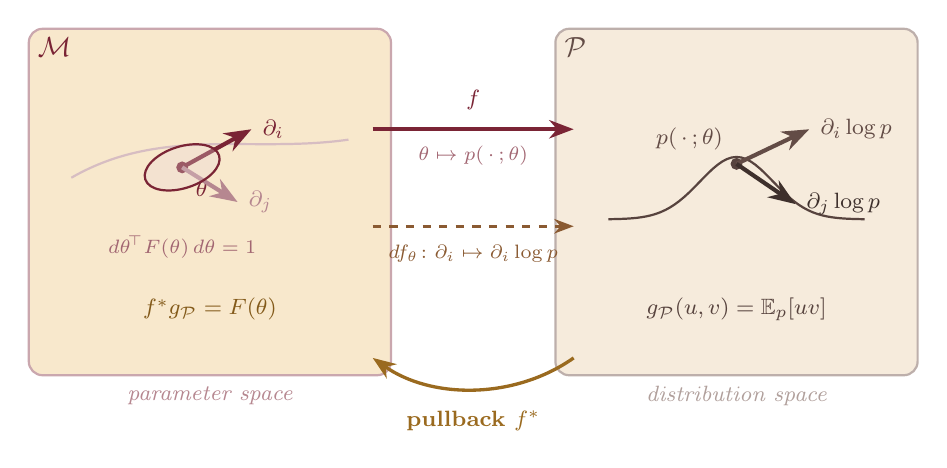
\begin{tikzpicture}[font=\small, scale=0.88]
 
  % ---- Left box M ----
  \node[mbox, minimum width=4.6cm, minimum height=4.4cm]
    (Mbox) at (0,0) {};
  \node[anchor=north west, deepblue, font=\normalsize\bfseries,
        inner sep=0] at ($(Mbox.north west)+(0.14,-0.14)$)
    {$\mathcal{M}$};
  \node[deepblue!55, font=\footnotesize\itshape]
    at ($(Mbox.south)+(0,-0.28)$) {parameter space};
 
  \draw[deepblue!30, thick]
    (-2.0, 0.35) .. controls (-0.7,1.1) and (0.6,0.7) .. (2.0, 0.9);
 
  \coordinate (th) at (-0.4, 0.5);
  \filldraw[deepblue] (th) circle (2.2pt);
  \node[deepblue, below right=2pt, font=\footnotesize] at (th)
    {$\theta$};
 
  \draw[tanvec, deepblue]    (th) -- ++(1.0, 0.55)
    node[right, font=\footnotesize] {$\partial_i$};
  \draw[tanvec, deepblue!55] (th) -- ++(0.8,-0.50)
    node[right, font=\footnotesize] {$\partial_j$};
 
  \draw[deepblue, thick, fill=lightblue, fill opacity=0.3,
        rotate around={18:(th)}] (th) ellipse (0.56cm and 0.30cm);
 
  \node[deepblue!70, font=\scriptsize] at (-0.4,-0.65)
    {$d\theta^{\!\top}F(\theta)\,d\theta=1$};
 
  \node[warmgold!85!black, font=\footnotesize\bfseries]
    at (0,-1.55) {$f^*g_{\mathcal{P}}=F(\theta)$};
 
  % ---- Right box P ----
  \node[pbox, minimum width=4.6cm, minimum height=4.4cm]
    (Pbox) at (7.6,0) {};
  \node[anchor=north west, softgreen!80!black,
        font=\normalsize\bfseries, inner sep=0]
    at ($(Pbox.north west)+(0.14,-0.14)$) {$\mathcal{P}$};
  \node[softgreen!60, font=\footnotesize\itshape]
    at ($(Pbox.south)+(0,-0.28)$) {distribution space};
 
  \begin{scope}[shift={(7.6,0)}]
    \coordinate (pfth) at (0.0, 0.55);
    \draw[softgreen!70!black, thick, domain=-1.85:1.85, samples=55]
      plot (\x, {0.90*exp(-1.8*\x*\x) - 0.25});
    \filldraw[softgreen!70!black] (pfth) circle (2.2pt);
    \node[softgreen!80!black, above left=2pt, font=\footnotesize]
      at (pfth) {$p(\,\cdot\,;\theta)$};
 
    \draw[tanvec, softgreen!80!black]
      (pfth) -- ++(1.05, 0.50)
      node[right, font=\footnotesize] {$\partial_i\log p$};
    \draw[tanvec, softgreen!50!black]
      (pfth) -- ++(0.85,-0.58)
      node[right, font=\footnotesize] {$\partial_j\log p$};
 
    \node[softgreen!70!black, font=\footnotesize\bfseries]
      at (0.0,-1.55) {$g_{\mathcal{P}}(u,v)=\mathbb{E}_p[uv]$};
  \end{scope}
 
  % ---- Map arrow f (above centre) ----
  \draw[mapsto]
    (2.35, 1.05) -- (5.25, 1.05)
    node[midway, above=3pt, font=\footnotesize\bfseries, deepblue]
      {$f$}
    node[midway, below=2pt, font=\scriptsize, deepblue!70]
      {$\theta\mapsto p(\,\cdot\,;\theta)$};
 
  % ---- Differential df (below centre) ----
  \draw[dfstyle]
    (2.35,-0.35) -- (5.25,-0.35)
    node[midway, below=3pt, font=\scriptsize, midblue]
      {$df_\theta\colon\partial_i\mapsto\partial_i\log p$};
 
  % ---- Pullback arc (below both boxes) ----
  \draw[pullbackarrow]
    (5.25,-2.25)
    .. controls (4.4,-2.85) and (3.2,-2.85) ..
    (2.35,-2.25)
    node[midway, below=4pt, font=\footnotesize\bfseries, warmgold]
      {pullback $f^*$};
 
\end{tikzpicture}
\end{document}
